\documentclass[compress, containsverbatim,mathserif, xcolor=dvipsnames, unicode]{beamer}
\usepackage[english, serbianc]{babel}

\usepackage{booktabs}
\usepackage{xcolor}
\usepackage{graphicx}

\mode<presentation>
{
\usetheme{Madrid}      
\usecolortheme{crane} 
\usefonttheme{serif} 
\setbeamertemplate{navigation symbols}{}
\setbeamertemplate{caption}[numbered]
}

\setbeamertemplate{footline}[frame number] 

\definecolor{cc-blue}{HTML}{1f77b4}
\definecolor{cc-orange}{HTML}{ff7f0e}
\definecolor{cc-green}{HTML}{2ca02c}
\definecolor{cc-red}{HTML}{d62728}
\definecolor{cc-purple}{HTML}{9467bd}

\title{Нигеријска превара\\\small{Рачунарство и друштво\\Математички факултет\\Универзитет у Београду}}
\author{Павле Савић\\mi17169@alas.matf.bg.ac.rs}
\date{
 \footnotesize{Београд, 2021.}
}


\begin{document}

\begin{frame}
\titlepage

\begin{figure}[h!]
    \centering
    \begin{flushleft}
    
\includegraphics[width=15mm]{slike/matf.png}
    \end{flushleft}
\end{figure}

\end{frame}

\begin{frame}{Увод}

\begin{itemize}		
	\item Превара 419 и нигеријски кривични законик
	\item Авансне провизије, лажне лутрије, црни новац
	\item Пошта -> Факс -> Е-пошта
	\item 419scam.org
	\item Различита у односу на нежељену пошту (eng. \emph{spam})
	\item 59\% нежељене поште садржи \emph{URL}-адресе
	\item Избегавање традицоналних \emph{spam} филтера е-поште
	\item 8\% нежељене поште чиниле су Преваре 419 (2009-2014)
\end{itemize}

\begin{figure}[h!]
    \centering
    \begin{center}
    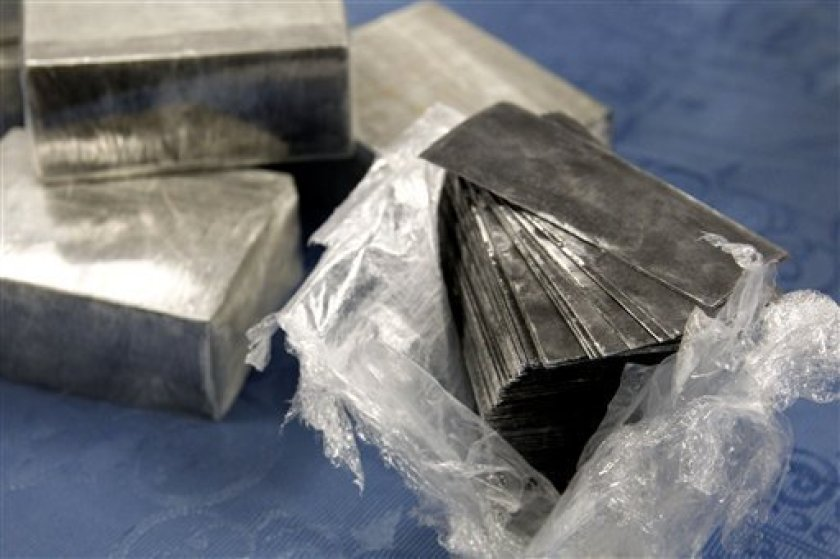
\includegraphics[width=50mm]{slike/blackmoney.jpg}
    \caption{Црни новац}
    \end{center}
\end{figure}

\end{frame}

\begin{frame}

\begin{figure}[h!]
    \centering
    \begin{center}
    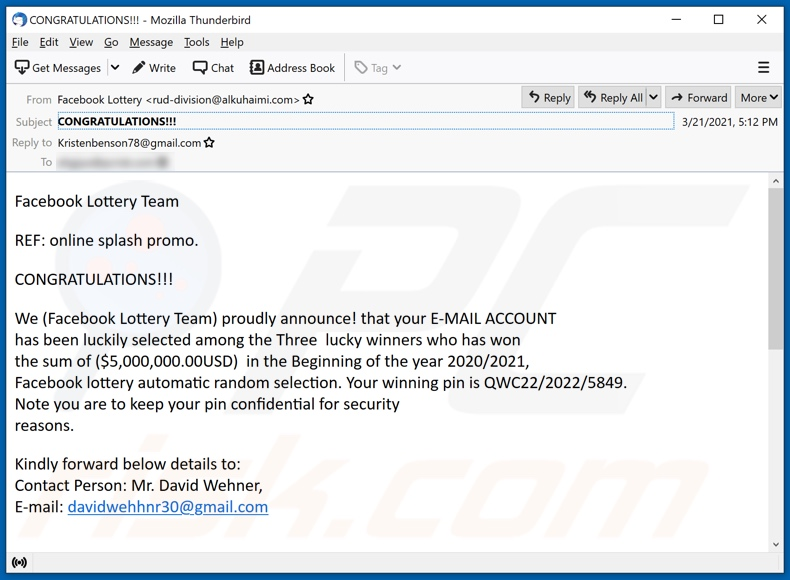
\includegraphics[width=50mm]{slike/fake.jpg}
    \caption{Лажна лутрија}
    \end{center}
\end{figure}

\begin{itemize}
	\item Употреба телефонских бројева током дужег периода потенцијално шанса за откривање \emph{скамера} 
	\item \emph{Кластеровање} - омогућује повезивање мејлова који деле заједничке особине, потенцијално припадају истој кампањи (?)
	\item Телефонски бројеви - камен темељац приликом повезивања 
	\item \emph{Macro-cluster}-и потенцијално указују на кампање већег обима
	\item \emph{Кластеровање} се експериментално показало као успешно и за истраге других шема сајбер криминала 	
\end{itemize}
	
\end{frame}

\begin{frame}

\begin{figure}[h!]
    \centering
    \begin{center}
    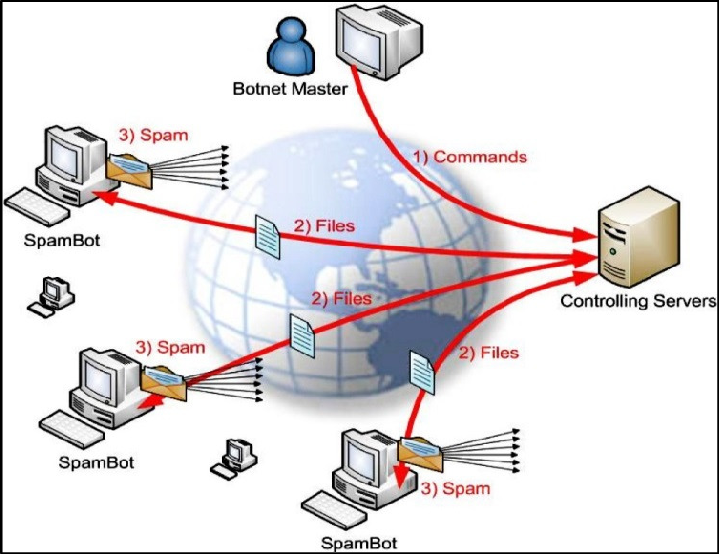
\includegraphics[width=25mm]{slike/botnet.png}
    \caption{Ботнет}
    \end{center}
\end{figure}

\begin{figure}[h!]
    \centering
    \begin{center}
    
\includegraphics[width=25mm]{slike/target.jpg}
    \caption{Циљани напад}
    \end{center}
\end{figure}

\begin{figure}[h!]
    \centering
    \begin{center}
    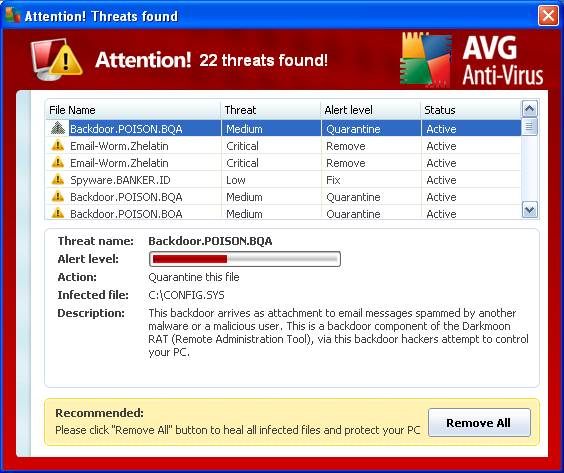
\includegraphics[width=25mm]{slike/avg.jpg}
    \caption{Лажни антивирус}
    \end{center}
\end{figure}

\end{frame}

\begin{frame}{Скуп података}

\begin{itemize}
	\item \emph{419scam.org - a 419 scam aggregator} (јануар 2009-август 2012.) претпроцесирани подаци
	\item Телефонски бројеви могу означавати географску локацију
	\item Бројеви мобилних телефона коришћени за нигеријску превару прецизно указују на државу пребивалишта нападача, пронађено неколико случајева роминга
\end{itemize}

\begin{table}[h!]
\begin{center}
\caption{Опште статистике}
\begin{tabular}{|c|c|} \hline
\textbf{Опис} & \textbf{Број} \\ \hline
Скам поруке & 36.761 \\ \hline
Јединствене поруке & 26.250\\ \hline
Укупно мејл адреса & 112.961\\ \hline
Јединствене мејл адресе & 34.723\\ \hline
Укупно телефонских бројева & 41.320\\ \hline
Јединствени телефонски бројеви & 11.768\\ \hline
Број држава & 12\\ \hline
\end{tabular}
\label{tab:tabela}
\end{center}
\end{table}

\end{frame}

\begin{frame}
\begin{itemize}
	\item Број адреса е-поште три пута већи од броја телефонских бројева
	\item Свака порука у скупу може садржати до 5 адреса е-адреса (\emph{from}, \emph{reply}, и адресе наведене у тексту поруке)
	\item Дистрибуција уједначена у посматраном трогодишњем периоду
	\item Скуп ограничен на европске и афричке регионе
	\item 71\% адреса е-поште коришћено је само током једног дана, преостале у просеку 79 дана
	\item 51\% телефонских бројева коришћено је само током једног дана, остатак у просеку 174 дана
	\item Телефонски број значајна особина приликом \emph{кластеровања}
\end{itemize}
\end{frame}

\begin{frame}
\begin{table}[h!]
\begin{center}
\caption{Телефони по државама}
\begin{tabular}{|c|c|c|} \hline
\textbf{Држава} & \textbf{Укупно телефона} & \textbf{Укупно (\%)}\\ \hline
Уједињено Краљевство & 4.499 & 43\\ \hline
Нигерија & 3.121 & 30\\ \hline
Бенин & 1.448 & 14\\ \hline
Јужна Африка & 562 & 5\\ \hline
Шпанија & 372 & 4\\ \hline
Холандија & 263 & 3\\ \hline
Обала Слоноваче & 89 & 1\\ \hline
Кина & 68 & 1\\ \hline
Сенегал & 47 & 0.5\\ \hline
Того & 11 & 0.1\\ \hline
Индонезија & 1 & 0.01\\ \hline
\end{tabular}
\label{tab:tabela2}
\end{center}
\end{table}
\begin{itemize}
	\item Сви бројеви из УК у скупу података припадају \emph{personal numbering services}
	\item Укупно у скупу 44\% \emph{personal numbering services} бројева, 44 \% бројева мобилних телефона, 12\% фиксних линија, мање од 1\% су непостојећи бројеви
\end{itemize}
\end{frame}


\begin{frame}
\begin{itemize}
	\item Порукама које су препознате као 419 превара се додељује и поткатегорија
	\item Категоризација врсте преваре заснива се на фреквенцији речи у порукама
	\item 64\% сврстано у категорију \emph{419 scam}, 24\% у категорију \emph{Fake lottery}
	\item \emph{Fake lottery} повезана са европским телефонским бројевима, код \emph{419 scam} порука нападачи користе подједнако често британске и нигеријске бројеве		
\end{itemize}
\end{frame}

\begin{frame}
\begin{figure}[h!]
    \centering
    \begin{center}
    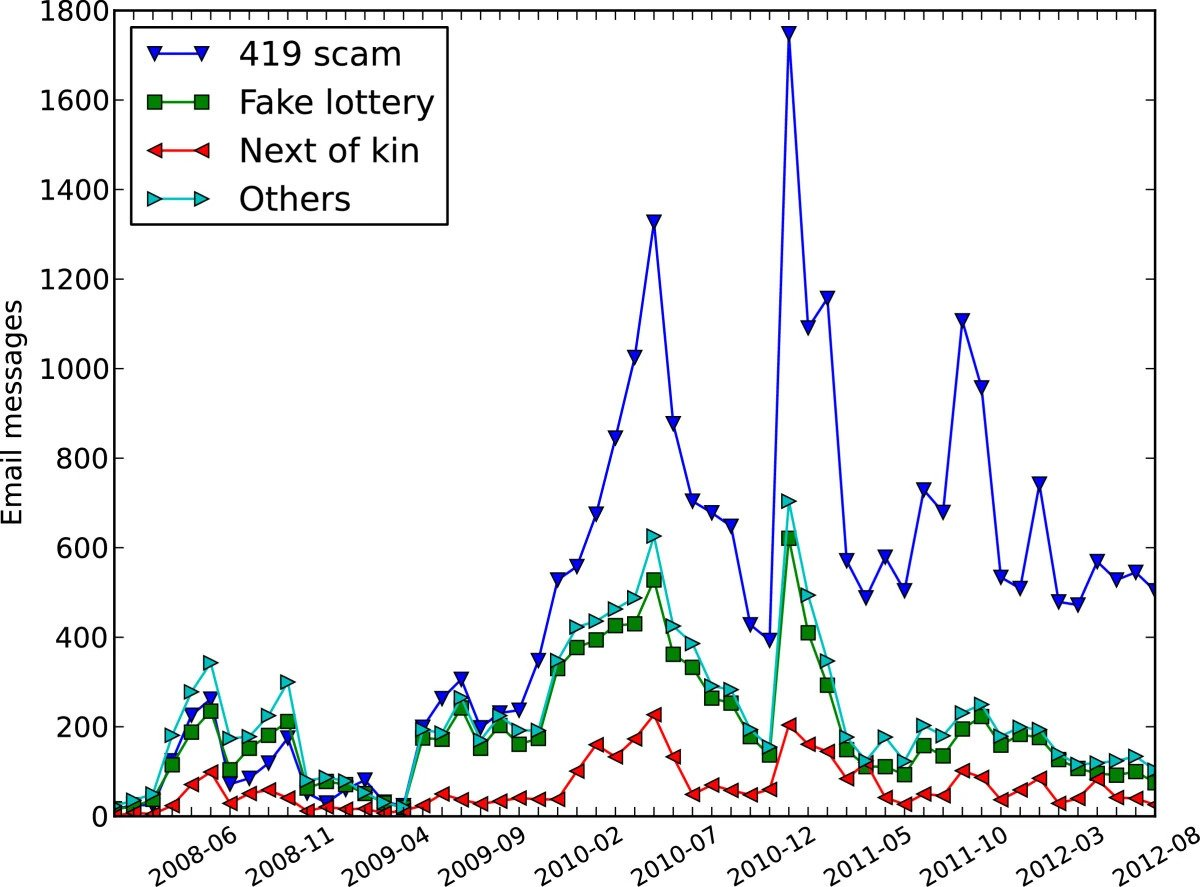
\includegraphics[width=47mm]{slike/1.jpg}
    \caption{Scam email categories over time}
    \end{center}
\end{figure}

\begin{figure}[h!]
    \centering
    \begin{center}
    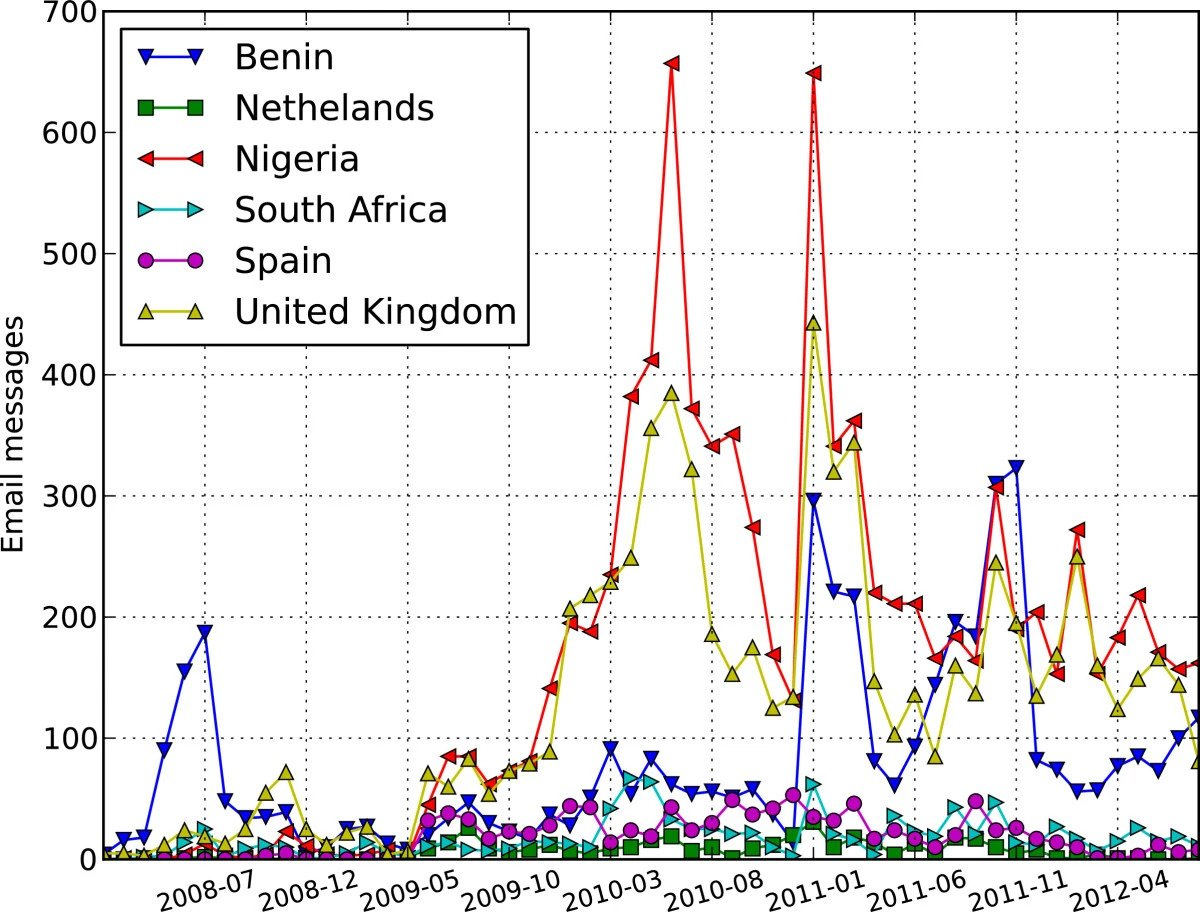
\includegraphics[width=47mm]{slike/2.jpg}
    \caption{\emph{419 scam} category phone numbers over time by countries}
    \end{center}
\end{figure}

\end{frame}

\begin{frame}{Методе анализе података}
\begin{itemize}
	\item Да би се идентификовале групе порука које имају изгледа да буду део исте кампање врши се \emph{кластеровање}
	\item Користи се \emph{TRIAGE} радни оквир за безбедносно истраживање података
	\item Критеријуми за груписање засновани на подскуповима заједничних особина
	\item \emph{TRIAGE} идентификује сложене обрасце у подацима што помаже при одређивању \textbf{тактика}, \textbf{техника} и \textbf{процедура} којима се нападачи служе
	\item \emph{TRIAGE} показао употребљивост и у контексту других безбедносних истрага	
\end{itemize}
\end{frame}

\begin{frame}
\begin{figure}[h!]
    \centering
    \begin{center}
    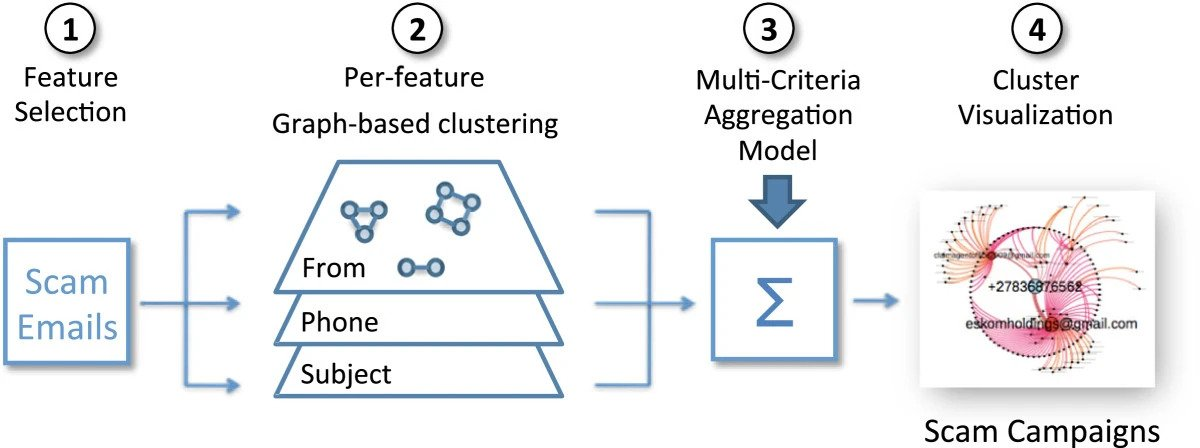
\includegraphics[width=75mm]{slike/3.jpg}
    \caption{\emph{TRIAGE} workflow on scam dataset}
    \end{center}
\end{figure}

\begin{itemize}
	\item Први корак - одабирање карактеристика (адреса е-поште пошиљаоца, наслов поруке, датум слања, адреса одговора, број телефона, адресе е-поште у телу поруке...)
	\item Други корак - грађење односа међу узорцима у односу на изабране особине користећи \textbf{метрике сличности}
\end{itemize}
\end{frame}

\begin{frame}
\begin{table}[h!]
\begin{center}
\caption{Weights of individual features (total = 1)}
\begin{tabular}{|c|c|} \hline
\textbf{Feature} & \textbf{Importance} \\ \hline
Phone & 0.30\\ \hline
From & 0.12\\ \hline
Reply & 0.18\\ \hline
Subject & 0.25\\ \hline
Email body & 0.1\\ \hline
Date & 0.05\\ \hline
\end{tabular}
\label{tab:tabela3}
\end{center}
\end{table}

\begin{itemize}
	\item Трећи корак - агрегирање појединачних сличности карактеристика, омогућено је додељивање тежина особинама
	\item Четврти корак - агрегирана вредност се користи као улаз за класичне \emph{graph clustering} алгоритме
	\item Дефинисање тежина према \emph{Regular Increasing Monotone - RIM} квантификатору омогућава нам да моделирамо стратегије 
\end{itemize}
\end{frame}
	
\begin{frame}{Резултати кластеровања}
\begin{itemize}
	\item Идентификовано 1.040 кластера који се састоје од најмање 5 скам порука
	\item Величине кластера у просеку мале, ово би могло одражавати тежњу скамера да остану \emph{испод радара}
\end{itemize}
\begin{table}[h!]
\begin{center}
\caption{Global statistics of the top 250 clusters}
\begin{tabular}{|c|c|c|c|} \hline
\textbf{Statistic} & \textbf{Average} & \textbf{Median} & \textbf{Maximum} \\ \hline
Number of emails & 38 & 28 & 376\\ \hline
Number of from & 13.9 & 9 & 181\\ \hline
Number of replies & 6.2 & 5 & 56\\ \hline
Number of subjects & 9.9 & 7 & 114\\ \hline
Number of phones & 2.5 & 2 & 34\\ \hline
Duration (in days) & 396 & 340 & 1.454\\ \hline
Number od dates(distinct) & 27.9 & 22 & 259\\ \hline
Compactness & 2.5 & 2.4 & 5.0\\ \hline
\end{tabular}
\label{tab:tabela4}
\end{center}
\end{table}		
\end{frame}

\begin{frame}{Процена резултата кластеровања}
\begin{itemize}
	\item Кластеровање је класификација без надзора, ваљаност резултата се процењује објективним критеријумима
	\item Екстерна и интерна валидација (\emph{Adjusted rand index})
	\item Испитана укупна компактност резултата, разврстана по појединачним карактеристикама
	\item Компактност је индекс ваљаности кластера који показује колико су кластери хомогени
	\item \emph{TRIAGE} чува све појединачне везе између сличних особина порука унутар кластера, на тај начин пружа увид у \emph{стабилне} карактеристике 
\end{itemize}
\end{frame}

\begin{frame}
\begin{table}[h!]
\begin{center}
\caption{Top coalitions of features across all clusters}
\begin{tabular}{|c|c|c|c|} \hline
\textbf{Coalition} & \textbf{Percentage (\%)}\\ \hline
(phone, subject, from, reply, email body) & 13\\ \hline
(phone, reply, email body) & 12\\ \hline
(phone, subject, reply, email body) & 11\\ \hline
(phone, from, reply, email body) & 7\\ \hline
(phone, subject) & 6\\ \hline
(phone, from) & 5\\ \hline
(phone, reply) & 4\\ \hline
(phone, reply, subject) & 4\\ \hline
(phone, reply, subject, from) & 4\\ \hline
others & 33\\ \hline
\end{tabular}
\label{tab:tabela5}
\end{center}
\end{table}
\begin{itemize}
	\item Особине одговорне за повезивање скам порука у кластерима укључује телефонске бројеве у 88\% случајева, \emph{reply} е-адресу у 66\% случајева, \emph{from} е-адресу у 46\% случајева	
\end{itemize}
\end{frame}

\begin{frame} {Макро-кластери}
\begin{itemize}
	\item Настају спајањем међусобно слабо повезаних кластера
	\item У нашем контексту, указују на могуће скам кампање већег обима, сачињене од међусобно слабо повезаних поткампањи вођених од стране истих нападача
	\item Значајне особине су само адресе е-поште и телефонски бројеви, тражени су кластери који деле најмање једну адресу е-поште и/или телефонски број
	\item Идентификован скуп од 845 изолованих кластера и други скуп од 195 повезаних кластера (62 макро-кластера)
	\item Ове везе шема одлучивања сматрала је преслабим, па су стога ти скамови груписани у одвојене кластере
	\item На аналитичару је да процени колико су такве везе заправо значајне
	\item Пракса је да се почне од скупа смислених кластера, а затим да се прагови постепено смањују до тачке у којој више нема основа за приписавање кампањи истој групи

\end{itemize}
\end{frame}

\begin{frame}{Закључак}
\begin{itemize}
	\item Телефонски бројеви и адресе е-поште имају кључну улогу у превари 419 за разлику од других шема сајбер криминала
	\item Нигерија и Велика Британија најзаступљеније државе порекла ових порука
	\item Велика разноликост начина увлачења жртве у превару и начина вођења кампање
	\item Скамери се труде да увек буду актуелни
\end{itemize}
\end{frame}

\end{document}
